% http://pgfplots.net/media/tikz/examples/TEX/mesh-plot.tex
\documentclass[border=10pt]{standalone}
%%%<
\usepackage{verbatim}
%%%>
\usepackage{pgfplots}
\pgfplotsset{width=7cm,compat=1.8}

\begin{comment}
:Title: Scatter plot with cubes
:Tags: 3D;Mesh plots;Manual
:Author: Christian Feuersänger
:Slug: mesh-plot

A mesh plot uses different colors for each mesh segment. The color is
determined using a "color coordinate" which is also called "meta data"
throughout this document. It is the same data which
is used for surface and scatter plots as well.

The code is from the PGFPlots 1.10 manual: "4.6.5 Mesh Plots".
\end{comment}

\begin{document}
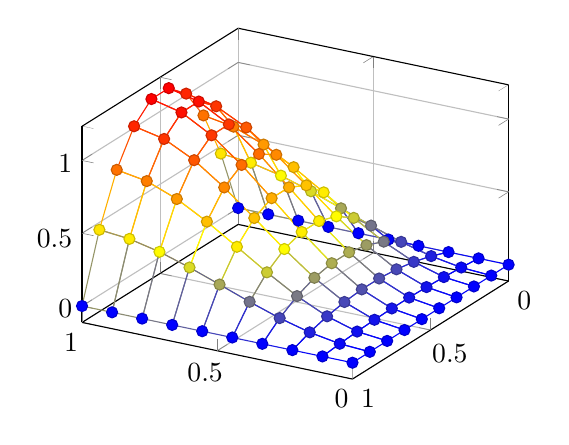
\begin{tikzpicture}
	\begin{axis}[grid=major,view={210}{30}]
	\addplot3+[mesh,scatter,samples=10,domain=0:1] 
		{5*x*sin(2*deg(x)) * y*(1-y)};
	\end{axis}
\end{tikzpicture}
\end{document}